\documentclass{article}

\usepackage{arxiv}

\usepackage[utf8]{inputenc} % allow utf-8 input
\usepackage[T1]{fontenc}    % use 8-bit T1 fonts
\usepackage{hyperref}       % hyperlinks
\usepackage{url}            % simple URL typesetting
\usepackage{booktabs}       % professional-quality tables
\usepackage{amsfonts}       % blackboard math symbols
\usepackage{microtype}      % microtypography
\usepackage{graphicx}
\usepackage{natbib}
\usepackage{doi}
\usepackage{listings}



\title{Quantifying uncertainty in Pareto estimates of global lake area}

%\date{September 9, 1985}	% Here you can change the date presented in the paper title
\date{} 					% Or removing it

\author{ \href{https://orcid.org/0000-0002-5924-2464}{
\includegraphics[scale=0.06]{orcid.pdf}\hspace{1mm}Jemma Stachelek} \\
	Earth System Observations\\
	Los Alamos National Laboratory\\
	Los Alamos, NM, USA, 87544 \\
	\texttt{jsta@lanl.gov} \\
}

% Uncomment to remove the date
%\date{}

% Uncomment to override  the `A preprint' in the header
%\renewcommand{\headeright}{Technical Report}
%\renewcommand{\undertitle}{Technical Report}
\renewcommand{\shorttitle}{Pareto lake area uncertainty}

%%% Add PDF metadata to help others organize their library
%%% Once the PDF is generated, you can check the metadata with
%%% $ pdfinfo template.pdf
\hypersetup{
pdftitle={Quantifying uncertainty in Pareto lake area estimates},
pdfsubject={stat.AP},
pdfauthor={Jemma Stachelek}
}

\begin{document}
\maketitle

\begin{abstract}
	Size is a critical factor determining the rate and occurrence of specific lake processes such as carbon sequestration and greenhouse gas emissions and emerging evidence suggests that small lakes in particular have particularly large $CO^2$ flux rates. Because we do not have a complete census of all lakes, upscaling estimates of such processes to small lakes at broad spatial scales requires the use of lake size-abundance distributions rather than empirical measurements of area. Existing lake census efforts are incomplete such that as lakes become smaller, they are more likely to be omitted either because they are too small to be resolved from remote sensing products or because of limited ground surveying effort (i.e. "censoring" of small lakes relative to large lakes). The present study explores one potential shortcoming of prior approaches estimating global lake area using lake size-abundance distributions. Namely, that these prior approaches rely on frequentist curve fitting techniques combined with an ad-hoc cutoff determination strategy (visual inspection to determine a likely censoring point). This yields an over-exact lake area estimate that is typically reported with no uncertainty bounds. I show how these shortcomings can be addressed with a Bayesian model that produces larger estimates of lake area uncertainty relative to the typical approach. When used as part of a sensitivity analysis, such an approach has the potential to enable more robust intercomparisons among studies of aquatic processes upscaling.
\end{abstract}

\section{Introduction}
Size is a critical factor determining the contribution of lakes to global biogeochemical cycling. As such, existing evidence suggests that lakes are key components of overall carbon burial, sequestration, and greenhouse gas emissions with small lakes having particularly high $CO^2$ flux rates \citep{delsontroGreenhouseGasEmissions2018, kellerGlobalCarbonBudget2021}. When upscaled to broad spatial extents, the high flux rates of these small lakes translate to a disproportionately large influence on overall $CO^2$ emissions \citep{piMappingGlobalLake2022}. The calculation of such fluxes requires two terms 1) an areal flux rate and 2) the distribution of total lake area. As with all quantitative estimates at broad spatial scales, uncertainty estimates are of great interest both because they allow for intercomparisons among similar studies and because they allow for comparisons between ecosystems.

The techniques typically used to determine uncertainty in areal flux rates differ greatly from those used to determine uncertainty in total lake area distributions. In the former case, uncertainties can typically be calculated in straightforward manner from literature compilations \citep{delsontroGreenhouseGasEmissions2018, kellerGlobalCarbonBudget2021}. In the latter case, uncertainty in total lake area distributions is challenged by the fact that no existing database is a complete census of all lakes \citep{messagerEstimatingVolumeAge2016} and the distribution of individual lake areas spans a range of approximately 7 orders of magnitude. The largest lakes are so big they could otherwise be classified as inland seas (> 104 $km^2$) while the smallest are barely larger than a regulation sized soccer (football) field (> $10^{-3}$ $km^2$).

A consequence of these challenges is that uncertainty varies within the distribution as a function of lake size. The area of the largest lakes is known with a high degree of certainty while the area of the smallest lakes is unknown below a certain unknown threshold. The area of a small lake can be unknown either because it is too small to be resolved from remote sensing products or because of limited ground surveying effort. The omission or "censoring" of small lakes occurs because we know that small lakes exist but below a certain threshold, we have limited knowledge of their exact areas \citep{hamiltonEstimationFractalDimension1992}. Such censoring errors may have an outsized impact on upscaled estimates of aquatic processes such as $CO^2$ flux because small lakes have been shown to have particularly large $CO^2$ flux rates \citep{delsontroGreenhouseGasEmissions2018,piMappingGlobalLake2022}.

Estimating total lake area from a sample of lakes requires a conceptual model of how lakes are formed (i.e. the data generating process). Typically, lake areas are treated as arising from a fractal generating process due to the fact that landform topography, which determines the placement of lakes, can itself be treated as a fractal generating process. Indeed, many other geomorphological phenomena that are dependent on landform topography such as coastline length are often well-described by fractal generating processes \citep{newman_power_2005}. A challenge in modelling such data generating processes for lake areas is that large lakes likely follow a different data generating process than that of the smallest lakes. Whereas small lakes are constrained by landform topography, large lakes are essentially unconstrained by local landform topography and are instead constrained by the placement and arrangement of continents \citep{goodchildLakesFractalSurfaces1988}. As large lakes become even larger, they have a greater probability of intersecting a continent edge and becoming an estuary or embayment rather than a lake. Consequently, lake databases are said to be truncated on large lakes because we know that large lakes are essentially fixed in space and cannot occur in any given location \citep{hamiltonEstimationFractalDimension1992}.

Given that no existing database is a complete census of all lakes, yet we have near exact estimates of the area of large lakes, estimating total lake area requires a method of dealing both with the fact that lake databases are 1) truncated at large lakes and 2) censored at small lakes. Prior studies estimating global lake area have mostly not dealt with the first issue (but see \citet{seekell2011does}). Note that in some instances the estimation process can be modified to limit its effect on the results (see Methods section). In contrast to the first issue, prior studies have typically addressed the second issue by specifying an ad-hoc cutoff value below which empirically determined lake areas are discarded and subsequently back-calculated. Hereafter, I refer to this strategy as the "cutoff" method.

In the present study, I explore two different methods for calculating uncertainty bounds around global lake area. First, I calculate these bounds using a frequentist approach for estimating total lake area (i.e. the cutoff method) via a simulation study. Second, I compare these frequentist uncertainty bounds with those calculated using a Bayesian framework. I carry out these demonstrations using a simulated dataset so that the ability of each method to recover the "true" parameter values can be evaluated. The use of a simulated dataset has the further benefit of avoiding potential confounding factors such as heterogeneity of survey effort or unknown data precision. The following analysis assumes that total global lake area has minimal temporal variability or at least minimal spatial trend. As a result, reported total lake areas can be thought of as “anticipated” or equilibrium long-run lake area rather than true totals representing any specific point in time. 


\section{Methods}

\subsection{Data description}

I compared the properties of a simulated dataset of lake areas (described below) against that of the HydroLAKES dataset \citep{messagerEstimatingVolumeAge2016}. HydroLAKES was created as a compilation of existing broad scale lake datasets including the SRTM Water Body Data \citep{slater2006srtm} and contains information on lakes between 0.1 and 500 $km^2$. The total area of the HydroLAKES dataset is 2.67 mil. $km^2$.

\subsection{Model overview}



Lake areas are typically treated as arising from a scale-invariant fractal generating process \citep{winslowDoesLakeSize2015, downingGlobalAbundanceSize2006, mcdonald_regional_2012, goodchildLakesFractalSurfaces1988, hamiltonEstimationFractalDimension1992}. This means that the number of lakes in one size class is proportional to the number of lakes in the preceding size class irrespective of their magnitudes. The numerical form describing such a process is a power-law function. One of the statistical tools often used to model data that follow a power-law function is the Pareto distribution which has a probability density function (pdf) of:

\begin{equation}
	pdf(A) = \alpha x_{min}^{\alpha}A^{-(\alpha+1)} \\
	\label{eqn:pareto_pdf}
\end{equation}

where $A$ is lake area, $a$ controls the “shape” of the distribution and $x_{min}$ controls the “scale” of the distribution \citep{shaliziAdvancedDataAnalysis2017}. Lake area studies using the Pareto distribution do not typically use the pdf directly. Instead, they use the inverse (complementary) cumulative distribution function (ccdf) (i.e. quantile function):

\begin{equation}
	ccdf(A) = \frac{x_{min}}{(1-A)^{\frac{1}{\alpha}}}
	\label{eqn:pareto_ccdf}
\end{equation}

The reason for using the ccdf is two-fold. First, it stabilizes model estimates in the lower tail of the distribution \citep{newman_power_2005}. This can be seen from the simulated data in Figure \ref{fig:pareto_demo} where the Pareto pdf contains a lot of noise in the tail but the ccdf appears smoothed. The smoothing of the tail is also desirable because it functions as a way of dealing with the truncated nature of lake databases (i.e. the area of large lakes is known exactly). The second reason for using the ccdf is that it provides a computational shortcut for estimating the Pareto shape parameter $a$ because it is numerically equivalent to the slope of the ccdf in log-log space \citep{downingGlobalAbundanceSize2006}.

\begin{figure}[h]
	\centering
	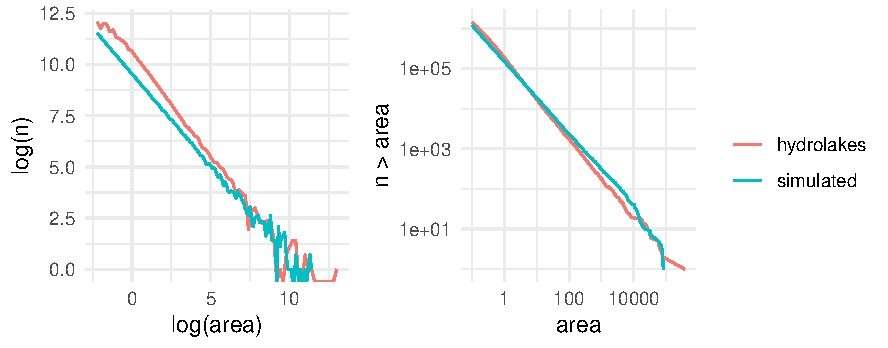
\includegraphics{figures/pareto_demo-1}
	\caption{Realization of a Pareto (A) probability density function and (B) complementary cumulative distribution function compared against equivalent calculations on the HydroLAKES dataset.}
	\label{fig:pareto_demo}
\end{figure}

For evaluation purposes, I generated a simulated dataset of 153,000 lake areas following the Pareto distribution using inverse transform sampling \citep{newman_power_2005}. Lakes in my simulated dataset have a minimum and maximum area of approximately 0.1 and 81,000 $km^2$ respectively. This maximum was chosen to be approximately as large as Lake Superior but less than the Caspian Sea following \citep{lehnerDevelopmentValidationGlobal2004}. The number of lakes in the simulated dataset was adjusted so that the total “true” area of the dataset (3.28 mil $km^2$) would approximately match (but still exceed) the total reported in the HydroLAKES dataset (2.93 mil $km^2$). I simulated a censored lake dataset by excluding approximately 60\% of lakes in the total dataset. I approximated the "true" lake area total by constructing the empirical distribution function (edf) of the data which approximates the underlying Pareto cdf \citep{newman_power_2005}. Then I used this estimate of the cdf slope to generate cdf estimates for the censored lakes. I combined these cdf estimates with the edf values from the known lakes before calculating the sum of the inverted distribution \ref{fig:predict_area}.

I estimated the Pareto shape parameter $a$ in a frequentist framework by calculating the the slope of the edf in log-log space using linear regression in \texttt{R} \citep{team2013r}. I evaluated uncertainty in both $a$ and total lake area in a Bayesian framework using Stan \citep{standevelopmentteamStanModelingLanguage2017}. Instead of computing on the edf (as in the frequentist case), I computed directly on the pdf with a Stan model \citep
[See][]{jemma_stachelek_2022_7459227}. I used uninformative gamma priors for both the $x_{min}$ and $a$ parameters following \citet{scollnikCompositeLognormalParetoModels2007}. I ran the model with four chains of 25,000 iterations and used the Stan defaults for thinning and burn-in which specify no thinning and discarding the first half (12,500) of iterations. I examined model fits to ensure that all models had acceptable convergence of MCMC chains.

Finally, I evaluated empirical uncertainty in total lake area using the size-dependent detection/non-detection estimates reported by \citet{cheruvelil2021lagos} which found that about 80\% of lakes $<$ 1 $km^2$ and 95\% of lakes between 1 and 10 $km^2$ were accurately represented in the US National Hydrograph Network. I implemented a random sampling (n=500) procedure using these detection fractions whereby empirical uncertainty is reported as the quantiles of the resulting distribution.

\section{Assessment}

The total area of the simulated dataset (3.28 mil. $km^2$, Table \ref{tab:area}) was larger than the empirical total of the HydroLAKES (2.67 mil. $km^2$) dataset. Visual inspection of the frequentist results, which are computed on the edf, appeared to produce a reasonable density estimate for small, censored lakes (Figure \ref{fig:predict_censor}). Although frequentist estimates of total lake area were close to the "true" value, uncertainty bounds were unrealistically small compared to an empirical estimate of uncertainty (Table \ref{tab:area}).

In contrast to the fixed a and fixed total lake area estimates produced by the frequentist approach, I found substantial variability in both a (95\% CI: 0.65, 1.02) and total area using a Bayesian approach (Figure \ref{fig:bayesian_model}, \ref{fig:bayesian_area}). In particular, the Bayesian 95\% credible intervals for a encapsulated the true value (Figure \ref{fig:bayesian_model}). Despite larger uncertainty estimates using a Bayesian approach (i.e. more closely matching the empirical estimate of uncertainty), the true value of total lake area was underestimated. The reason for this underestimation is likely owed to incomplete “back calculation” in the cutoff method (i.e. back calculated lakes did not extend all the way to the smallest lakes in the simulated dataset).


\begin{figure}
	\centering
	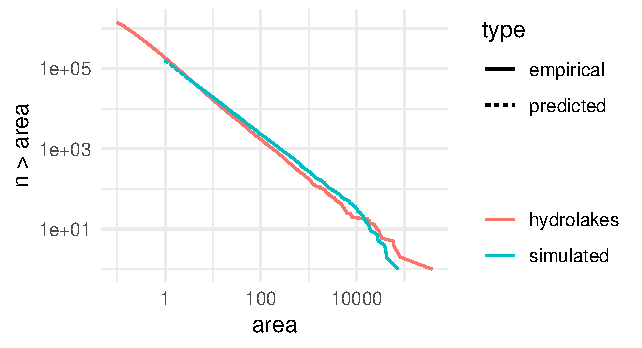
\includegraphics{figures/predict_censor-1}
	\caption{Simulated lake area (purple line) where the portion calculated from the edf (>= 0.1 $km^2$) is denoted by a solid line and the portion calculated from the transformed cdf (< 0.1 $km^2$) is denoted by a dashed line. For comparison, the edf of the HydroLAKES dataset (solid yellow line) is also shown.}
	\label{fig:predict_censor}
\end{figure}

\begin{table}
	\caption{Comparison between the true total lake area in the simulated dataset against frequentist and Bayesian estimates. The true total is a point estimate while uncertainty is displayed via differences between the 95th and 5th quantile.}
	\centering
	\begin{tabular}{lllll}
		\toprule
		& Q50 (mil $km^2$) & Q5 (mil $km^2$) & Q95 (mil $km^2$) & Q95-Q5 \\
		\midrule
		True (point estimate) & 3.278 & - & - & - \\
		True (80\% non-detect) & 3.205 & 3.205 & 3.205 & 673  \\
		Frequentist & 3.274 & 3.274 & 3.274 & 14  \\
		Bayesian & 3.199 & 3.158 & 3.273 & 115172 \\
		\bottomrule
	   \end{tabular}	
	\label{tab:area}
\end{table}

\begin{figure}
	\centering
	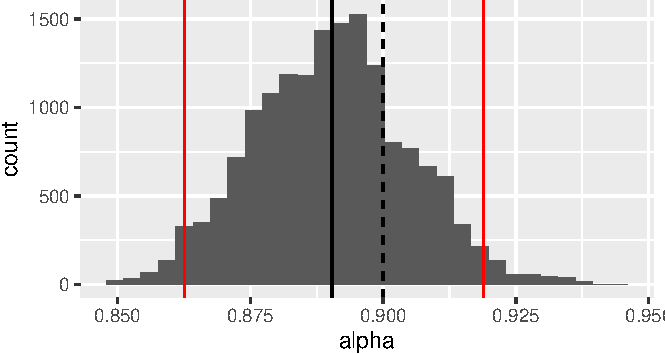
\includegraphics{figures/bayesian_model-1}
	\caption{Median (black line) and central 95 percent interval estimates of alpha (red lines). Here the 'true' alpha is 0.9.}
	\label{fig:bayesian_model}
\end{figure}

\begin{figure}
	\centering
	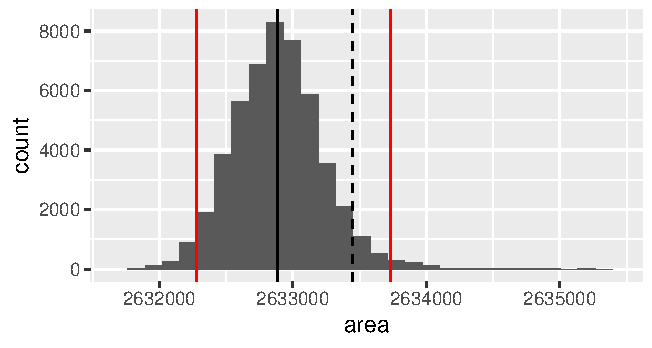
\includegraphics{figures/bayesian_area-1}
	\caption{Median (black line) and central 95 percent interval estimates of total lake area (red lines). Here the true total lake area is marked with a dashed vertical line.}
	\label{fig:bayesian_area}
\end{figure}

\section{Discussion}

I have shown that the even with realistic estimates of the density of small censored lakes, the typical frequentist cutoff method does not reasonably capture uncertainty in total lake area (Table \ref{tab:area}). However, the results of the Bayesian approach by contrast, indicate substantial uncertainty in both total lake area and the underlying Pareto shape parameter a used to derive these estimates (Figure \ref{fig:bayesian_model}, \ref{fig:bayesian_area}). The combination of accurate lake area accounting and realistic uncertainty estimates offered by this approach may provide a more principled way to assess the relative influence of different lake area classes on global lake fluxes ($CO^2$, $CH^4$, etc.)  beyond ad-hoc study intercomparisons or even meta-analysis on collections of prior studies.

The Bayesian model estimate of total lake area was an underestimate of the true total lake area of the simulated datasets (Figure \ref{fig:bayesian_area}). Some of this underestimation is because the Pareto shape parameter a was estimated from the truncated dataset (to simulate the fact that observed datasets such as HydroLAKES have some unknown degree of truncation) and was lower ({\raise.17ex\hbox{$\scriptstyle\mathtt{\sim}$}}0.82) than the true value of 0.9. This lower value of a resulted in lower than expected total lake area. Such underestimation would increase with a greater proportion of censoring. Another likely contributor to lake area underestimation is differences in the properties of the simulated data compared to an empirical dataset like HydroLAKES. Note that the simulated dataset diverges notably from HydroLAKES for the largest waterbodies because these are few in number such that randomness in the simulation is more obvious (Figure \ref{fig:pareto_demo}). Taken together, these factors (i.e. less and less truncation and better data on the largest waterbodies) may explain the steady increase in estimates of global lake area through time from approximately 3 to 5 million $km^2$ as lake area databases have improved their accuracy \citep{downingGlobalAbundanceSize2006,lehnerDevelopmentValidationGlobal2004,verpoorterGlobalInventoryLakes2014}. Future work on estimating global lake area may consider implementing a sensitivity analysis looking at the response of total area estimates to variation in the degree of censoring.

Another area where further sensitivity analyses may be warranted is in the generation of total lake area estimates from Pareto realizations. Typically this is done a single time such that any particular reported estimate comes only from a single realization. To generate the simulated dataset for the present study, I generated multiple realizations with the goal of arriving at one that approximately matched the total reported in HydroLAKES. Although each realization matched the Pareto properties of HydroLAKES, the sum of many of the realizations differed markedly from each other and from HydroLAKES. This demonstrates the need for generating multiple Pareto estimates of total lake area for aquatic process upscaling as part of a sensitivity analysis rather than taking only a single realization.

A caveat of the present study is that it is difficult to confirm whether or not any particular dataset follows a fractal generating or Pareto process without strong prior knowledge. As a result, there is some degree to which we cannot know whether the distribution of lake areas truly aligns with the Pareto distribution \citep{seekell2011does}. Indeed data following many heavy-tailed distributions such as the lognormal or negative exponential can appear to be equivalent to power-law distributions such as the Pareto \citep{clausetPowerlawDistributionsEmpirical2009,seekell2011does}. The results of the present study confirm that an apparent change in the shape of the lower tail of a lake area distribution does not necessarily indicate a change in the data generating process. Note that the simulation dataset analyzed herein is a truly fractal generated dataset with a homogeneous data generating process, yet a cursory look would seem to indicate a change of data-generating process in the lower tail (Figure \ref{fig:predict_censor}).

In addition to a sensitivity analysis of censoring, future work might consider more complex models that treat lake areas as a mixture of a Pareto distribution for small lakes and either a negative exponential or lognormal distribution for large lakes. Such an approach has been demonstrated by \citep{bonabeau_scaling_1999-1} and \citep{scollnikCompositeLognormalParetoModels2007}. Both studies show that the point at which the distribution mixtures converge can provide valuable inference. In the case of lakes, such a convergence point may indicate a change in the data generating process such as the point at which lake areas are controlled by continent placement rather than fractal landscape morphology \citep{goodchildLakesFractalSurfaces1988,hamiltonEstimationFractalDimension1992}. Knowing such a convergence point would provide a data-driven estimate of what constitutes a “large lake” beyond ad-hoc cutoffs and supplement existing definitions based on hydrodynamics and circulation.


% \begin{minipage}[c]{0.95\textwidth}
% 	\begin{lstlisting}
% data {
%   int<lower=0> N;
%   real x[N];
% }
% parameters {
%   real<lower=0> alpha;
%   real<lower=0> xmin;
% }
% model {
%   real lpa[N];

%   xmin ~ gamma(.001, .001);
%   alpha ~ gamma(.001, .001);

%   for (i in 1:N) {
%     lpa[i] = pareto_lpdf(x[i] | xmin, alpha);
%   }

%   target += sum(lpa);
% }
% \end{lstlisting}
% \end{minipage}

\bibliographystyle{jsta}
\bibliography{pareto-lakes}

\end{document}
